\documentclass{beamer}
\usepackage{ccicons}
\usepackage{hyperref}
\usepackage{minted}

% ❤️ https://github.com/elauksap/focus-beamertheme
\usetheme{focus}
\title{Reactive Applications\\in Frontend Engineering Today}
\author{Manuel Alabor}
\institute{Master Seminar\\HSR University of Applied Sciences Rapperswil}
\date{}

\setminted{autogobble=true, tabsize=2, linenos=false, frame=single, breaklines=true}

\begin{document}

\begin{frame}
	\maketitle
	\Tiny{\ccby\thinspace\thinspace This work is licensed under a \href{https://creativecommons.org/licenses/by/4.0/}{Creative Commons Attribution 4.0 International License}}.
\end{frame}

% \begin{frame}{Overview}
% 	\tableofcontents
% \end{frame}

\section*{Welcome}

\begin{frame}{Motivation and Goals}
	\begin{itemize}
		\item Get acquainted with scientific research work style\bigskip
		\item Review a research report\bigskip
		\item Transfer topic to the field of frontend engineering\bigskip
		\item Write a research report\bigskip
	\end{itemize}
\end{frame}

\begin{frame}[focus]
	``On the Positive Effect of Reactive Programming on Software Comprehension: An Empirical Study''
	\\\bigskip
	\small{Salvaneschi et al. \cite{7827078}}
\end{frame}


\subsection*{Research Questions}

\begin{frame}{RQ1: Design Sciences and \\Empirical Software Engineering}
	\begin{itemize}
		\item \textbf{RQ1.1} Which empirical research methods, approaches and concepts were applied by Salvaneschi et al. \cite{7827078}?\bigskip
		\item \textbf{RQ1.2} Are these research methods, approaches and concepts applied well, what could have been done better?\bigskip
		\item \textbf{RQ1.3} Do Salvaneschi et al. \cite{7827078} meet FAIR principles \cite{2019arXiv190805986H} \cite{wilkinson:2016} with their work?
	\end{itemize}
\end{frame}

\begin{frame}{RQ2: Software Engineering Principles}
	\begin{itemize}
		\item \textbf{RQ2.1} How do Salvaneschi et al. \cite{7827078} define RP and OOP?\bigskip
		\item \textbf{RQ2.2} When should RP be considered, and when not?\bigskip
		\item \textbf{RQ2.3} Which experiments should be conducted in future work?\bigskip
		\item \textbf{RQ2.4} Which design alternatives exist in the context of frontend engineering?
	\end{itemize}
\end{frame}


\section{Terminology}
\subsection*{Empirical Software Engineering}
\begin{frame}{Empirical Software Engineering}
	\begin{itemize}
		\item Lack of scientific and analytical formalism\bigskip
		\item Apply empirical research methods instead
	\end{itemize}
\end{frame}

\subsection*{Design Sciences}
\begin{frame}{Design Sciences}
	\begin{itemize}
		\item Research principle to grow research projects\bigskip
		\item Design and investigate on artifacts in a specific context\bigskip
		\item Iterate until stakeholders are satisfied
	\end{itemize}

	\begin{figure}
		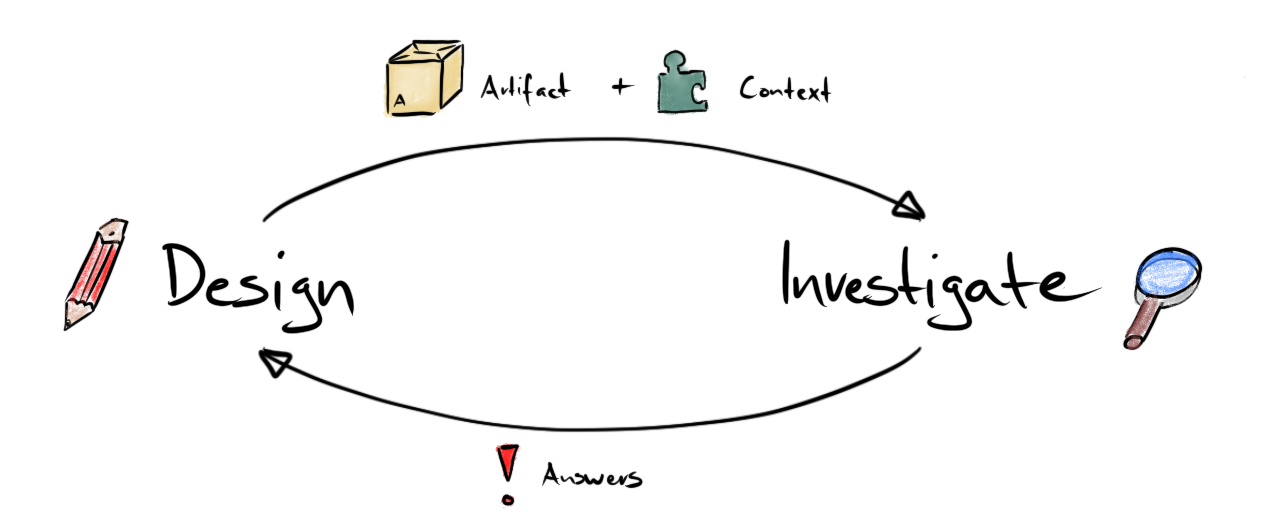
\includegraphics[width=.8\textwidth]{assets/slides/design-sciences-process.png}
	\end{figure}
\end{frame}

\subsection*{FAIR Research Principles}
\begin{frame}{FAIR Research Principles}
	\begin{itemize}
		\item \textbf{F}indability\bigskip
		\item \textbf{A}ccessibility\bigskip
		\item \textbf{I}nteroperability\bigskip
		\item \textbf{R}eusability
	\end{itemize}
\end{frame}

\subsection*{Reactive Programming}
\begin{frame}{Reactive Programming I}
	\begin{itemize}
		\item Declarative programming paradigm\bigskip
		\item Originated in functional programming\bigskip
		\item Describe values, their transformation and how they depend on each other over time\bigskip
	\end{itemize}
\end{frame}

\begin{frame}[fragile=singleslide]{Reactive Programming II}
	\textbf{TODO: Create Graphic}

	\begin{minted}{JavaScript}
		const currentDateString = Bacon
			.fromPoll(1000, () => new Date())
			.map(d => d.toISOString());
	\end{minted}
\end{frame}

\subsection*{Observer Design Pattern}
\begin{frame}{Observer Design Pattern \cite{gamma1995design}}
	\begin{columns}[t, onlytextwidth]
		\column{0.5\textwidth}
			\begin{itemize}
				\item Decouple components while maintaining communication between them\bigskip
				\item Originated in object oriented programming\bigskip
			\end{itemize}

		\column{0.5\textwidth}
			\textbf{TODO Create Graphic}
	\end{columns}
\end{frame}

\section{Review of Salvaneschi et al.}

\subsection{Study Overview}

\subsection{Study Result Overview}

\subsection{Review Results}

\section{Transfer to\\Frontend Engineering}

\begin{frame}

\end{frame}


\section{Conclusion}
\begin{frame}[focus]
	Questions?
\end{frame}

\begin{frame}[focus]
	Discussion
\end{frame}

\appendix
% \begin{frame}[allowframebreaks]{References}
\begin{frame}{References}
	\bibliographystyle{plain}
	\bibliography{bibliography}
\end{frame}

\end{document}